\documentclass{article}
\usepackage{amsmath, amsfonts, amssymb, amsthm, stmaryrd}
\usepackage{enumitem}
\usepackage{hyperref}
\usepackage{bbm}
\usepackage[ruled,linesnumbered]{algorithm2e}

\usepackage[verbose=true,letterpaper]{geometry}
\newgeometry{
  textheight=9.5in,
  textwidth=6.5in,
  top=0.5in,
  headheight=12pt,
  headsep=25pt,
  footskip=30pt
}
\setlength{\parskip}{0.5em} % blank lines between paragraphs
\usepackage{tikz}
\usepackage{pgfplots}

%%%%%% Commands and theorems
\theoremstyle{plain}
\newtheorem{Theorem}{Theorem}
\newtheorem{Proposition}{Proposition}
\newtheorem{Corollary}{Corollary}
\newtheorem{Lemma}{Lemma}

\theoremstyle{remark}
\newtheorem{Definition}{Definition}
\newtheorem{Assumption}{Assumption}
\newtheorem*{remark}{Remark}

\renewcommand{\P}{\mathbb{P}}
\newcommand{\E}{\mathbb{E}}
\newcommand{\R}{\mathbb{R}}
\newcommand{\N}{\mathbb{N}}
\renewcommand{\S}{\mathfrak{S}}

\newcommand{\sign}{\text{sign}}
\newcommand{\1}{\mathbbm{1}}
\newcommand{\id}{\mathrm{id}}

\newcommand{\argmin}{\arg\min}
\newcommand{\dec}{\,{\buildrel d \over =}\,}

\usepackage{color}
\usepackage{array}
\newcolumntype{L}[1]{>{\raggedright\let\newline\\\arraybackslash\hspace{0pt}}m{#1}}
\usepackage{todonotes}
\newcommand{\todoT}[1]{\todo[inline,color=blue!40]{{\textbf{T:}~}#1}}

\usepackage{enumitem}

% Have descriptions with italic and bullets:
\setlist[description]{font=\normalfont\itshape\textbullet\space}
% To include the section number in the equation numbering:
\numberwithin{equation}{section}

\title{Adaptive stopping in sequential tests to compare Deep RL Agents and improve replicability at low computational cost}
\date{}
\begin{document}
\maketitle
\section{Introduction}
%According to the ACM (Association for Computing Machinery), \textit{reproductibility} of a scientific study dictates that   ``An experimental result is not fully established unless it can be independently reproduced". Recently, the machine learning community witnessed a major crisis of reproductibility (see \cite{pineau2021improving} for Machine Learning in general and \cite{agarwal2021deep,colas2018many,colas2019hitchhiker} for Reinforcement Learning).
 In Reinforcement Learning (RL), a given experiment may sometimes take several days to run, and given the fact that the runs give random results, one needs to do several repetitions of the experiments and use statistical methods to control the efficiency of the algorithm. If one does not do enough repetitions and if the statistical methodology is not sound, the results of the experiment will not be reproducible and the results of the article are then called into question. In the present paper, we give a \textit{theoretically sound} statistical methodology to choose \textit{adaptively} the number of runs when comparing \textit{multiple RL agents} using the smallest number of runs possible.

\todoT{Continue introduction}

The usual methodology , we often use Monte-Carlo methods to evaluate the performances of an algorithm. In particular, if we denote $e(A)$ some evaluation of algorithm $A$, the global score of an algorithm by
$$S(A)=\frac{1}{N}\sum_{i=1}^N e_i(A) $$
where $e_1(A), \dots,e_N(A)$ are the evaluation of the algorithm $A$ on $N$ different seeds (i.e. $e_1(A),\dots,e_N(A)$ are supposed i.i.d).

\subsection{Current methodology in RL}
\paragraph{Theoretically sound study of Atari environments?}

Atari and Procgen environments are famous environment benchmark in Deep-RL. In these environments, the study is a bit different and often one may use very few seeds for one given game (typically 3 seeds) and compare the agents on a lot of different games. The comparisons are then aggregated by saying that algorithm $A_1$ is better than algorithm $A_2$ on more than $20$ games over the $26$ games considered. The statistic methodology behind this kind of aggregation is complicated because the reward distribution are not the same over each game and hence the comparisons are not identically distributed. Typically  this means that Agent $A_2$ may be better than Agent $A_1$ only on games that are hard, and $A_1$ is better on all the other, does this means that $A_1$ is a better algorithm than $A_2$? To our knowledge, there have not been any proper statistical guarentee for this kind of comparison. Aggregation of comparisons on several games in Atari is still an \textit{open problem} and it is \textit{outside the scope of this article}. In this article we suppose that we compare the agents only on one given task.

\paragraph{Theoretically sound comparison of multiple agents?}

One of the problem often encountered in the statistical method to compare several RL agents is the problem of comparing more than two agents. Indeed, statistical theory dictates that when doing a comparison between a lot of agent (multiple testing), then we need more sample from each agents' than if we compare only two agents. The basic idea is that there are a lot more occasions to make an error than when we compare only two agents, hence we need more data to have a lower probability of error at each comparison.

This informal argument is made precise when using multiple testing, but the theory of multiple testing have never been used to compare RL agents to our knowledge, we remedy this with our algorithm giving a theoretically sound workflow to compare a large number of RL agents.

\paragraph{How many random seeds for Mujoco environments?}
\todoT{Explain seeds, make reference to agrawal et al. and to sigaud}

\begin{figure}[h]
  \begin{center}
    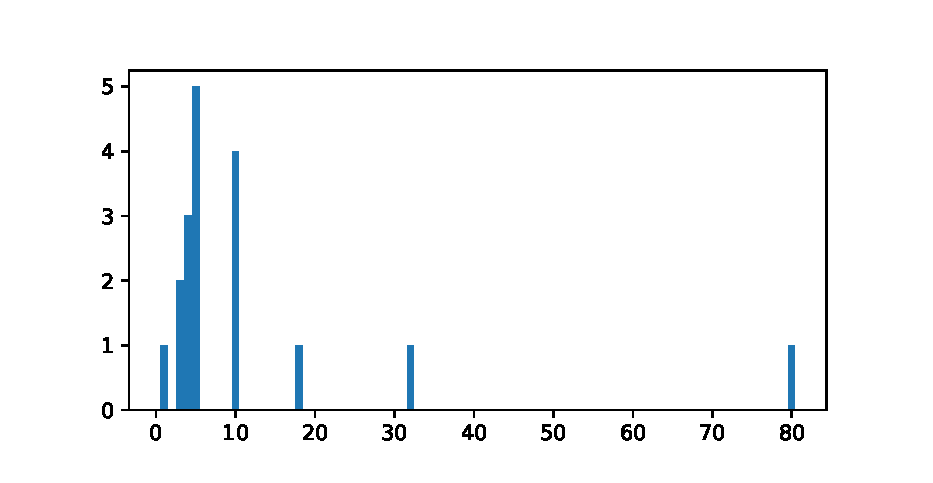
\includegraphics[width=0.8\textwidth]{census_icml2022.eps}
    \caption{Census of the number of seeds used in RL articles to study environments using Mujoco. From ICML 2022 articles.}
  \end{center}
\end{figure}

\subsection{Goal and requirements on the algorithm}

The goal of this article is, given two agents $A_1$ and $A_2$, to evaluate how high $N$ must be to be certain that either $\E[e_1(A_1)]=\E[e_2(A_2)]$ or $\E[e_1(A_1)]\neq \E[e_2(A_2)]$, i.e. do the two algorithms perform similarly or is one better than the other ? This is a trade-off between computational time and the need to assess correctly the scores of $A_1$ and $A_2$. The main properties that we want for our algorithm are as follows:

\begin{description}
\item[Multiprocessing] The algorithm should be able to treat batch of datas.
\item[Non-Parametric] The algorithm should be non-parametric.
\item[Fixed Budget] The algorithm should have a fixed maximum number of iterations used.
\item[Sample efficient] The algorithm should stop as soon as possible in practice.
\end{description}

One algorithm that verifies all the properties listed above is a group sequential permutation test that we will describe in this article.
\subsection{The shape of reward in Deep-RL problems}
\todoT{Have histograms of rewards for several very different agent/env pairs}
 
\subsection{Alternative approaches}
\paragraph{Non adaptive approaches}
\todoT{Talk about H2G2 and edge of statistical precipice}

\paragraph{Fully Sequential testing}
In the sequential testing setting, the data are handled one after the other, there is no batch of data. This is not adapted to our problem because in practice, one is often capable of training several agents in parallel, hence the evaluations are received by batch.

\paragraph{SPR/GLR test}
A particular class of sequential test often used are the Sequential Probability Ratio test and the Generalized Likelihood Ratio test. Both of these tests could be generalized to a group-sequential context but they both depend strongly on a parametric model for the data. However, the reward distribution of RL algorithms is often heavy-tail and multi-modal and as a consequence it is difficult to use a parametric model to represent all of them efficiently and simultaneously for several agents, each with a different reward distribution. Moreover, because we want to deal with small sample-sizes, the asymptotic of the central limit theorem is not adapted.

\paragraph{Bandits (Best arm identification or Ranking)} Our objective is close to the objective of ranking bandits algorithms. However compared to bandits we want to at the same time \textit{minimize the stopping time} (similar to fixed-confidence setting) of the algorithm and have a \textit{fixed maximum budget} (similar to fixed-budget setting). In our algorithm we allow for a type I error of $\alpha \in (0,1)$, which is very similar to the fixed confidence setting while still having a fixed budget. Then, compared to the fixed budget setting we allow a larger error rate and as a consequence we are more sample efficient than bandits algorithms.

\section{Description of the different tools used in the algorithm}
\subsection{Group sequential testing}

To choose $N$ adaptively, we propose to use group sequential testing (GST). GST are used in particular in clinical trials in which case an early stopping is desirable when comparing two drugs. We choose to use GST in particular and not sequential testing because the data are often naturally grouped due to the parallelization of the computation.

GST often suppose strong models on the data, in particular it is often supposed that the data are i.i.d. from a Gaussian distribution. This assumption is often not verified in the case of $e_i(A)$ being evaluations from a RL algorithm. In particular, the distribution of $e_i(A)$ often presents several modes and it can sometimes contain outliers.

The presence of several modes in the distributions of the evaluations and the difficulty to make any distributional assumption justify a non-parametric approach of the problem, but to further justify this approach we did a study of the effect of model misspecification on simulated data when using Gaussian GST algorithm.

\todoT{Explain early accept also} 

\subsection{Permutation tests}
Permutation tests are non-parametric tests that are exact for testing the equality in distribution. This means that the type I error of the test is controlled by $\alpha$ the parameter of the test.

Let us recall the basic formulation of a two-sample permutation test. Let $X_1,\dots,X_N$ be i.i.d from a law $P$ and $Y_1,\dots,Y_N$ i.i.d from a law $Q$, we want to test $P=Q$ against $P \neq Q$. Let $Z_i = X_i$ if $i\le N$ and $Z_i = Y_i$ if $i>N$, $Z_1,\dots,Z_{2N}$ is the concatenation of $X_1^N$ and $Y_1^N$. Then, the test proceeds has follow: we reject $P=Q$ if $T(\id) = \left| \frac{1}{N}\sum_{i=1}^N(Z_i-Z_{N+i})\right|$ is larger than more that $95\%$ of the values $T(\sigma) =  \left| \frac{1}{N}\sum_{i=1}^N(Z_{\sigma(i)}-Z_{\sigma(N+i)})\right|$ when $\sigma$ enumerates all the possible permutations of $\{1,\dots,N\}$. The idea is that if $P$ is different from $Q$, then $T(\id)$ should be large and on the other hand if we shuffle the data having that there are data both from $P$ and from $Q$ in the first half and in the second half then the difference of mean $T(\sigma)$ will be closer to zero.

Remark that in the main algorithm, we use Monte-Carlo approximation in that we use random permutation instead of enumerating all the permutations to estimate the quantiles.

\subsubsection{Multiple testing}
When dealing with multiple testing, particular care must be taken so as not to decrease the error of the test. Suppose that we want to test $H_j$ versus $H_j'$ for $1\le j\le J$ using a test statistic $T_{N}^{(j)}$. Instead of the type I error considered in two-sample testing, we consider the family-wise error rate (FWE) which is defined as the probability of making at least one type I error: let $\textbf{I}\subset \{1,\dots,J\}$ be the set of the true hypotheses, then 
$$\mathrm{FWE} = \P_{H_j, j \in \textbf{I}}\left(\exists j \in \textbf{I}:\quad  \text{reject }H_j \right).$$
Usually, we say that an algorithm has a weak FWE control if the FWE is smaller than $\alpha$ when $\textbf{I}=\{1,\dots,J\}$ and we say that the algorithm has strong FWE control if FWE is smaller than $\alpha$ for any $\textbf{I}\neq \emptyset$.

There are several procedures that can be used to have control on the FWE. The most famous one is Bonferroni procedure, it is a very simple procedure in which we take a threshold for $H_j$ vs $H_j'$ equal to a quantile of order $1-\alpha/J$ of the permutation distribution of $T_n^{(j)}$. It can be very conservative in general and we will prefer a step-down method that performs better in practice.

\paragraph{Step-down procedure:} proposed by \cite{Romano_2003}, the step-down procedure is defined as follows: for some $\textbf{C} \subset \{1,\dots,J\}$, denote
$$T_{n}^{(\textbf{C})}(\sigma)= \max\left(T_n^{(j)}(\sigma),\quad j \in \textbf{C}\right),$$
and the threshold of the test $\widehat{b}_{n}^{(\textbf{C})}$ is defined as the quantile of order $1-\alpha$ of the permutation law of $T_{n}^{(\textbf{C})}(\sigma)$:
\begin{equation}\label{eq:threshold_multi} 
\widehat{b}_{n}^{(\textbf{C})} = \inf\left\{b>0: \frac{1}{(2n)!} \sum_{\sigma \in \S_{2n}} \1\{T_{n}^{(\textbf{C})}(\sigma) \ge b\} \le   \alpha  \right\}.
\end{equation}
\begin{algorithm}[h]
\SetAlgoLined
\SetKwInput{KwParameter}{Parameters}
\KwParameter{$\alpha \in (0,1)$}
Initialize $\textbf{C}=\{1,\dots,J\}$\\
\While{$\textbf{C} \neq \emptyset$}{
Compute $\widehat{b}_{n}^{(\textbf{C})}(1-\alpha)$  from Equation~\eqref{eq:threshold_multi}.\\
\uIf{$T_{n}^{(\textbf{C})}(\mathrm{id}) \le \widehat{b}_{n}^{(\textbf{C})}$}{
Accept all the hypotheses $H_j, j\in \textbf{C}$ and break the loop.}
\Else{
Reject $H_{j_{\max}}$ where $j_{\max} =  \arg\max\left(T_n^{(j)}(\sigma),\quad j \in \textbf{C}\right)$.\\
Define $\textbf{C}=\textbf{C} \setminus \{j_{max}\}$
}
}
\caption{Multiple testing, non-sequential.}\label{alg:multiple_test_1}
\end{algorithm}
The Algorithm~\ref{alg:multiple_test_1} is consistent (i.e. $\mathrm{FWE}\le \alpha$) for the equality of distribution hypotheses. It uses the maximum of the statistics as a mean to test an intersection of hypotheses. This procedure is not specific to permutation tests and can be used for other tests provided some properties on the thresholds $\widehat{b}_{n}^{(\textbf{C})}$. 

Remark that we could not use Benjamini-Hochberg procedure or similar procedures because the hypotheses are not independent. We adapt this procedure to the case of group sequential testing in Section~\ref{sec:main_algo}

\section{Simple case of two agents without early accept}
We denote by $\S_{2N}$ the set of permutations of $\{1,\dots,2N\}$ and for $\sigma_1,\sigma_2,\dots,\sigma_k \in \S_{2N}^2$, we denote $\sigma_1^k=\sigma_1 \cdot \sigma_2 \cdot \ldots \cdot \sigma_k$ the concatenation of the permutation $\sigma_1$ done in interim $1$ and $\sigma_2$ done on interim $2$,\dots, $\sigma_k$ on interim $k$.

In the case where only two agents are compared, we use the following algorithm (see Section~\ref{sec:multi} for the multi-agent and fully developped version of the algorithm). We denote 
$$T_{N,i}(\sigma_1^k)= \left|\sum_{i=1}^k\left(\sum_{n=1}^{N} e_{\sigma_i(n),i}(A_1)-\sum_{n=N+1}^{2N} e_{\sigma_i(n),i}(A_2)\right)\right|,$$
and the boundary 
\begin{equation}\label{eq:bound_2}
\widehat{b}_{N,k}\in \inf\left\{b >0 : \frac{1}{((2N)!)^k}\sum_{\sigma_1^k \in S_k} \1\{T_{N,k}(\sigma_1^k) \ge  b\} \le  \frac{\alpha}{K}\right\} .
\end{equation}
where $S_k$ is the set of permutations $\sigma_1^k\in(\S_{2N})^k$  such that it would not have rejected before
$$\forall m < k,\quad  T_{N,m}(\sigma_1^k) \le   \widehat{b}_{N,m} $$
The algorithm is as follows 
\begin{algorithm}[h]
\SetAlgoLined
\SetKwInput{KwParameter}{Parameters}
\KwParameter{Agents $A_1,A_2$, environment $\mathcal{E}$, number of blocks $K \in \N^*$, size of a block $N$, level of the test $\alpha\in (0,1)$.}
Define $2NK$ different seeds $s_{1,1},\dots,s_{1,N},s_{2,1},\dots,s_{2,N}$.\\
\For{$k=1,\dots,K$}{
\For{$i=1,2$}{
Train agent $A_i$ on environment $\mathcal{E}$ with the seeds $s_{i,kN},\dots,s_{i,(k+1)N}$.\\
Collect evaluations $e_{1,k}(A_i),\dots,e_{N,k}(A_i)$ using this trained agent.\\
}
Compute the boundary $\widehat{b}_{N,k}$ from Equation~\eqref{eq:bound_2}.\\
\If{$T_{N,k}(\id) \ge \widehat{b}_{N,k}$}{
Reject the equality of the agents' evaluation, break the loop.
}
\Else{
If $k=K$ then accept, otherwise continue.
}
}
If the test was never rejected, return accept. Else return reject.
\caption{Adaptive Stopping, two agents without early accept.}\label{alg:adastop_2}
\end{algorithm}

An illustration of the group sequential test is given in figure~\ref{fig:gst}. The boundary in blue is computed sequentially to have a final level $1-\alpha$ for the test, the red points are the observed values of the test statistic (denoted $w_i$). The algorithm stops at the third iteration $k=10$ because the observed value of $w_i$ is outside the boundary.

\begin{figure}
\begin{center}
% This file was created with tikzplotlib v0.10.1.
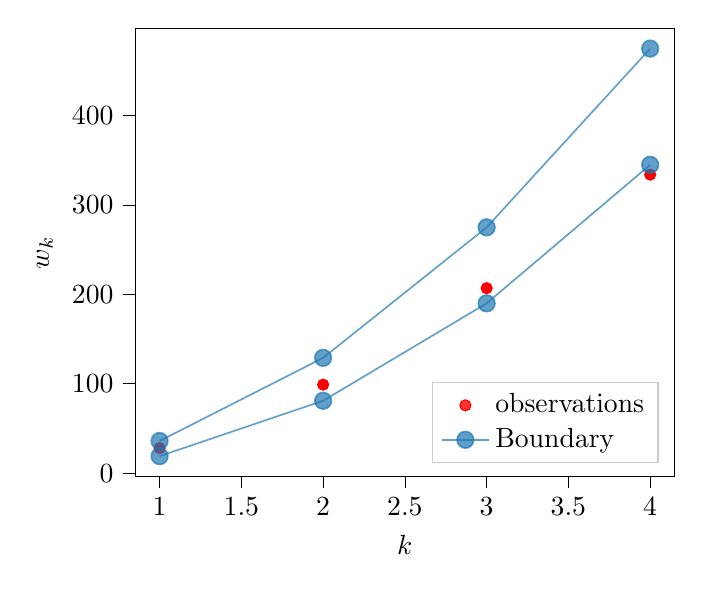
\begin{tikzpicture}

\definecolor{darkgray176}{RGB}{176,176,176}
\definecolor{lightgray204}{RGB}{204,204,204}
\definecolor{steelblue31119180}{RGB}{31,119,180}

\begin{axis}[
legend cell align={left},
legend style={
  fill opacity=0.8,
  draw opacity=1,
  text opacity=1,
  at={(0.97,0.03)},
  anchor=south east,
  draw=lightgray204
},
tick align=outside,
tick pos=left,
x grid style={darkgray176},
xlabel={\(\displaystyle k\)},
xmin=0.85, xmax=4.15,
xtick style={color=black},
y grid style={darkgray176},
ylabel={\(\displaystyle w_k\)},
ymin=-3.8, ymax=497.8,
ytick style={color=black}
]
\addplot [draw=red, fill=red, mark=*, only marks]
table{%
x  y
1 28
2 99
3 207
4 334
};
\addlegendentry{observations}
\addplot [semithick, steelblue31119180, opacity=0.7, mark=*, mark size=3, mark options={solid}]
table {%
1 19
2 81
3 190
4 345
};
\addlegendentry{Boundary}
\addplot [semithick, steelblue31119180, opacity=0.7, mark=*, mark size=3, mark options={solid}, forget plot]
table {%
1 36
2 129
3 275
4 475
};
\end{axis}

\end{tikzpicture}

\caption{Illustration of the boundary for two agents.\label{fig:gst}}
\end{center}
\end{figure}



\subsection{General case with multiple agents}\label{sec:multi}

\subsubsection{Notations}
 We consider $L\ge 2$ agents $A_1,\dots,A_L$. The $k^{th}$ step of the algorithm is called the $k^{th}$ interim for some $k \in \{1,\dots,K\}$. Let $c_1,\dots,c_J$ be the comparisons we want to make. For any $i$, $c_i$ is a couple of agent's indices: $c_i=(c_{i,1},c_{i,2}) \in \{1,\dots,L\}^2$. We denote $e_{1,k}(j), \dots, e_{2N, k}(j)$ the concatenation of the $2N$ evaluations obtained from the two agents compared for comparison $j$ at at interim $k$.

For some $\textbf{C} \subset \{1,\dots,J\}$, denote
$$T_{N,k}^{(\textbf{C}^+)}(\sigma_1^k)= \max\left(T_{N,k}^{(j)}(\sigma_1^k),\quad j \in \textbf{C}\right) \quad \text{and}\quad T_{N,k}^{(\textbf{C}^-)}(\sigma_1^k)= \min\left(T_{N,k}^{(j)}(\sigma_1^k),\quad j \in \textbf{C}\right)$$
where 
$$T_{N,k}^{(j)}(\sigma_1^k)= \left|\sum_{i=1}^k\left(\sum_{n=1}^{N} e_{\sigma_i(n),i}(j)-\sum_{n=N+1}^{2N} e_{\sigma_i(n),i}(j)\right)\right|$$ 
$T_{N,k}^{(j)}$ is the absolute value of the sum of differences of all the blocks until block $i$ after permutation of the concatenation of the two agents's evaluations by $\sigma_1,\dots,\sigma_k\in \S_{2N}$.
 
$\textbf{I}$ denotes the set of indices of the true hypotheses among $\{1,\dots,J\}$. If $\textbf{I} \neq \emptyset$, we denote 
$$\mathrm{FWE}(\alpha) = \P\left(\exists j \in \textbf{I}:\quad  \text{reject }H_j \right).$$
\subsubsection{AdaStop: adaptive stopping algorithm using step-down method and group sequential permutation tests}\label{sec:main_algo}

The algorithm is given in Algorithm~\ref{algo:main} and depends on the values of the boundary thresholds. 
Instead of using all the permutations as it was done previously when comparing two agents, on may also use random permutations $s_1,\dots,s_B$ where each $s_i$ is a concatenation of $k$ permutations, $s_i\in(\S_{2N})^k$. The theoretical guarentees persist as long as the choice of the permutations is made independently of the data. Switching to random permutations allows us to use the algorithm for a larger array of values of $K$ and $N$. Using a small number of permutations will decrease the total power of the test, but with a sufficiently large number of random permutations (typically for the values of $N$ and $K$ considered, 10 000 permutations are sufficient) the loss in power is acceptable.

In the sequels, we will deote $B_k$ the number of concatenated permutations (random or not) considered at interim $k$. Then, with these permutations, we define the alternative boundary values $\widehat{b}_{N,k}^{(\textbf{C}^+)}$ and $\widehat{b}_{N,k}^{(\textbf{C}^-)}$ such that
\begin{equation}\label{eq:boundary_1}
\widehat{b}_{N,k}^{(\textbf{C}^+)} = \inf \left\{b >0 :\frac{1}{B_k}\sum_{\sigma \in S_k} \1\{T_{N,k}^{(\textbf{C}^+)}(\sigma_1^k) \ge  b\} \le  q_k\right\} 
\end{equation}
and
\begin{equation}\label{eq:boundary_2}
\widehat{b}_{N,k}^{(\textbf{C}^-)} = \sup\left\{ b>0 : \frac{1}{B_k}\sum_{\sigma \in S_k} \1\{T_{N,k}^{(\textbf{C}^-)}(\sigma_1^k) \leq b\} \le  q'_k \right\} .
\end{equation}
where $\sum_{j=1}^kq_j \le \frac{k\alpha}{K}$ and  $\sum_{j=1}^kq'_j \le \frac{k\beta}{K}$ and where $S_k$ is the subset of $\{s_1,\dots,s_{B_k}\}$ such that it would not have accepted or rejected before: for each $\sigma_1^k \in S_k$, we have the following property
$$\forall m < k,\quad  T_{N,m}^{(\textbf{C}^+)}(\sigma_1^k) \le   \widehat{b}_{N,m}^{(\textbf{C}^+)} \text{ and }T_{N,m}^{(\textbf{C}^-)}(\sigma_1^k) \ge   \widehat{b}_{N,m}^{(\textbf{C}^-)}.$$

\begin{algorithm}[h!]
\SetAlgoLined
\SetKwInput{KwParameter}{Parameters}
\KwParameter{Agents $A_1,A_2,\dots, A_L$, environment $\mathcal{E}$, comparison pairs $(c_i)_{i \le L}$ where $c_i$ is a couple of two agents that we want to compare. Integers $K,N \in \N^*$, test parameters $\alpha,\beta$.}
Define $LNK$ different seeds $(s_{l,n,k})_{l\le L,n\le N, k\le K}$.\\
Set $\textbf{C}=\{1, \dots,L\}$ the set of indices for the comparisons we want to do.\\
\For{$k=1,\dots,K$}{
\For{$l=1...L$}{
Train agent $A_l$ on environment $\mathcal{E}$ with the seeds $s_{l,1,k},\dots,s_{l,N,k}$.\\
Collect the $N$  evaluations of agent $A_l$.\\
}
\While{True}{
Compute the boundaries $\widehat{b}_{N,k}^{(\textbf{C}^+)}$ and $\widehat{b}_{N,k}^{(\textbf{C}^-)}$ from~\eqref{eq:boundary_1} and~\eqref{eq:boundary_2} .\\
\uIf{$T_{N,k}^{(\textbf{C}^+)}(\mathrm{id}) > \widehat{b}_{N,k}^{(\textbf{C}^+)}$}{
Reject $H_{j_{\max}}$ where $j_{\max} =  \arg\max\left(T_{N,k}^{(j)}(\id),\quad j \in \textbf{C}\right)$.\\
Update $\textbf{C}=\textbf{C} \setminus \{j_{\max }\}$
}
\uElseIf{$T_{n,k}^{(\textbf{C}^-)}(\mathrm{id}) < \widehat{b}_{N,k}^{(\textbf{C}^-)}$}{
Accept $H_{j_{\min}}$ where $j_{\min} =  \arg\min\left(T_{N,k}^{(j)}(\id ),\quad j \in \textbf{C}\right)$.\\
Update $\textbf{C}=\textbf{C} \setminus \{j_{\min }\}$
}
\Else{
Break the while loop.
}
}
\lIf{$\textbf{C}=\emptyset$}{
Break the loop and returns the answers.
}
{
\lIf{ $k=K$}{
 Then accept all hypotheses remaining in $\textbf{C}$.
}
}
}
\caption{Main algorithm\label{algo:main}}
\end{algorithm}



\newpage

\subsection{Theoretical guarentees}
% \todoT{For now: asymptotic is not with early accept and not multiple.}
% \todoT{
% TODO:\\
% - Prove that early accept does not decrease the power too much\\
% - Do the asymptotic for early accept and multiple testing (this would also allow estimate of power)
% } 
\subsubsection{Basic results following from the use of permutation tests}
One of the basic property of two-sample permutation tests is that when the null hypothesis is true, then all the permutation are as likely to give a certain value and hence the law given the data is the uniform distributions on all the permutations. Then, as a consequence of our choice of $\widehat{b}_k$ as a quantile of the law given the data, the algorithm has a probability to reject wrongly of $\alpha$. This informal statement is the result presented in the following theorem.


\begin{Theorem}\label{th:multi_FWE}
Suppose that $\alpha,\beta \in  (0,1)$, and consider the multiple testing problem $H_j: P_j = P_k$ against $H_j': P_j \neq P_k$ for all the couples $j \neq k$. 
Then, the test resulting from Algorithm~\ref{algo:main} has a strong control on the Family-wise error for the multiple test, i.e. if we suppose that all the hypotheses $H_i, i\in \bf I$ are true and the remainder are false, then 
$$ \P\left(\exists j \in \bf{I}:\quad  \text{reject }H_j\right)\le\alpha.$$
\end{Theorem}



 The proof for theorem for this result is a bit technical. In what follows we begin by showing the result in a very simplified case with $L=2$ agents, and $K=1$.
\begin{Lemma}\label{lem:quantile_permu_2}
  Let $X_1,\dots,X_N$ be i.i.d from a distribution $P$ and $Y_1,\dots,Y_N$ be i.i.d. from a distribution $Q$. Denote $Z_1^{2N}=X_1,\dots,X_N,Y_1,\dots,Y_N$ be the concatenation of $X_1^N$ and $Y_1^N$. Let $\alpha \in (0,1)$ and define $\widehat{b}$ such that 
  $$ \frac{1}{(2N)!}\sum_{\sigma\in \S_{2N}} \1\left\{ \frac{1}{N}\sum_{i=1}^n (Z_{\sigma(i)}-Z_{\sigma(N+i)}) > \widehat{b}\right\}\le \alpha.$$
  Then, if $P=Q$, we have 
  $$\P\left(\frac{1}{N}\sum_{i=1}^n (X_i-Y_i) >\widehat{b} \right)\le \alpha $$ 
\end{Lemma}
\begin{proof}
  Denote $T(\sigma)= \frac{1}{N}\sum_{i=1}^n (Z_{\sigma(i)}-Z_{\sigma(n+i)})$. Since $P=Q$, for any $\sigma,\sigma' \in \S_{2N}$ we have $T(\sigma)\dec T(\sigma')$. Then, because $\widehat{b}$ does not depend on the permutation $\sigma$ (but it depends on the values of $Z_1^{2N}$, we have for any $\sigma \in \S_{2N}$
  \begin{align*}
    \P\left(T(\id)> \widehat{b}\right)&=\P\left(T(\sigma)> \widehat{b}\right)
  \end{align*} 
  Now, take the sum on all the permutations, 
  \begin{align*}
    \P\left(T(\id)> \widehat{b}\right)&=\frac{1}{(2N)!}\sum_{\sigma\in \S_{2N}} \E\left[\1\{T(\sigma)> \widehat{b}\}\right]\\
                                      &=  \E\left[\frac{1}{(2N)!}\sum_{\sigma\in \S_{2N}}\1\{T(\sigma)> \widehat{b}\}\right]\le \alpha
  \end{align*}
  which proves the result.
\end{proof}

Denote 
$$\mathrm{NR}_k(\sigma_1^k) = \left\{\forall m < k,\quad  T_{N,m}^{(\textbf{I}^+)}(\sigma_1\cdot\ldots\cdot\sigma_m) \le   \widehat{b}_{N,m}^{(\textbf{I}^+)}\right\}$$
$\mathrm{NR}_k(\sigma_1^k)$ is the event on which the statistics corresponding to true hypotheses, computed after permutation by $\sigma_1^k=\sigma_1\cdot \ldots \cdot \sigma_k$, are not rejected.

Let $\textbf{I}$ be the set of true hypotheses. Let E be the following event
$$\mathrm{E}= \{ \exists j \in \textbf{I}: \quad H_j \text{ is rejected}\}.$$
Contrary to Lemma~\ref{lem:quantile_permu_2}, we are in a multiple-testing framework and there may be a mix of true hypotheses and false hypotheses and we have to reduce the problem to studying only true hypotheses because we don't have any informations on the distributions when the hypotheses are false. We also have to take into account the possibility to accept a true hypothesis early. We dennote by $\widehat{\bf I}_k \subset \bf I$ the set of true hypotheses not yet accepted at interim $k$.
\begin{Lemma}\label{lem:multiple_test_FWE}
We have 
$$\mathrm{FWE} = \P_{\sigma_1^k}\left(\mathrm{E}\text{ is true} \right) \le \sum_{k=1}^K\P\left( T_{N,k}^{(\widehat{\textbf{I}}_k^+)}(\id) > \widehat{b}_{N,k}^{(\widehat{\textbf{I}}_k^+)}, \mathrm{NR}_k(\id)\right)  $$
\end{Lemma}
Then, similarly as in the proof of Lemma~\ref{lem:quantile_permu_2}, because we managed to reduce the problem to consider only true hypotheses thanks to Lemma~\ref{lem:multiple_test_FWE}, we want to use the invariance by permutation to make the link with the definition of $\widehat{b}_{N,k}^{(\textbf{I}^+)}$. For this purpose, we prove the following Lemma.


\begin{Lemma}\label{lem:invariance}
We have that for $k \le K$, for any ${\sigma_1^k}$ concatenation of $k$ permutations, 
$$(T_{N,l}^{(\widehat{\bf{I}}_l^+)}(\id),\widehat{b}_{N,l}^{(\widehat{\bf{I}}_l^+)})_{l\le k}=(T_{N,i}^{(\widehat{\bf{I}}_l^+)}(\sigma_1^l), \widehat{b}_{N,l}^{(\widehat{\bf{I}}_l^+)})_{l\le k}$$
\end{Lemma}
Using Lemma~\ref{lem:invariance}, we have for any ${\sigma_1^k}$
$$\P\left(T_{N,k}^{(\widehat{\textbf{I}}_k^+)}(\id) > \widehat{b}_{N,k}^{(\widehat{\textbf{I}}_k^+)}, \mathrm{NR}_k(\id ) \right) = \P\left(T_{N,k}^{(\widehat{\textbf{I}}_k^+)}({\sigma_1^k}) > \widehat{b}_{N,k}^{(\widehat{\textbf{I}}_k^+)}, \mathrm{NR}_k({\sigma_1^k}) \right)$$

Hence, from Lemma~\ref{lem:multiple_test_FWE}, and Lemma~\ref{lem:invariance},
\begin{align*}
\mathrm{FWE} &\le \sum_{k=1}^K\frac{1}{B_k}\sum_{i=1}^{B_k}\P\left(T_{N,k}^{(\widehat{\textbf{I}}_k^+)}(s_i) > \widehat{b}_{N,k}^{(\widehat{\textbf{I}}_k^+)}, \mathrm{NR}_k(s_i) \right)\\
&= \sum_{k=1}^K\E\left[\frac{1}{B_k}\sum_{i=1}^{B_k}\1\left\{ T_{N,k}^{(\widehat{\textbf{I}}_k^+)}(s_i) > \widehat{b}_{N,k}^{(\widehat{\textbf{I}}_k^+)}, \mathrm{NR}_k(s_i)\right\} \right]\\
&= \sum_{k=1}^K \E\left[\frac{1}{B_k}\sum_{{\sigma_1^k} \in S_k}\1\left\{ T_{N,k}^{(\widehat{\textbf{I}}_k^+)}({\sigma_1^k}) > \widehat{b}_{N,k}^{(\widehat{\textbf{I}}_k^+)}\right\} \right]\\
&\le \sum_{k=1}^K q_k \le \alpha
\end{align*}
where we used the definition of $\widehat{b}_{N,k}^{(\widehat{\textbf{I}}_k^+)}$ to make the link with $\alpha$


% \newpage
\section{Simulated experiments}

\section{Comparison with non-adaptive approaches}
\todoT{Comparison with edge of statistical precipice and Flower's team article}

\appendix

\section{Proof of Lemmas}

% \paragraph{Proof that what I wanted to use do not work}
% Consider the case $N=2$, $L=3$ agents. Then, we have 
% $$T_{N,1}^{(1,2)}(\id)=|e_{1,1}(A_1)+e_{1,2}(A_1)-e_{1,1}(A_2)-e_{1,2}(A_2)| $$
% $$T_{N,1}^{(2,3)}(\id)=|e_{1,1}(A_3)+e_{1,2}(A_3)-e_{1,1}(A_2)-e_{1,2}(A_2)| $$
% $$T_{N,1}^{(1,3)}(\id)=|e_{1,1}(A_1)+e_{1,2}(A_1)-e_{1,1}(A_3)-e_{1,2}(A_3)| $$
% that we represent by the matrix
% \[
%   M = 
%   \begin{pmatrix}
%     1 & 1 & -1 & -1 & 0 & 0 \\
%     0 & 0 & -1 & -1 & 1 & 1 \\
%     1 & 1 & 0 & 0 & -1 & -1 \\
%   \end{pmatrix}
% \]
% and $T(M)=(T^{(1,2)}(\id),T^{(2,3)}(\id), T^{(1,3)}(\id)) = M\cdot(e_{1,1}(A_1),e_{1,2}(A_1),e_{1,1}(A_2),e_{1,2}(A_2),e_{1,1}(A_3),e_{1,2}(A_3) )^T$.
 
% One simple rule:  multiplying a line of $M$ by $-1$ does not change the value of $T(M)$.

% Consider the permutation 
% \[
%   \sigma = 
%   \begin{pmatrix}
%     1 & 2 & 3 & 4\\
%     3 & 1 & 2 & 4 
%   \end{pmatrix}
% \]
% with representation
% \[
%   M_\sigma = 
%   \begin{pmatrix}
%     -1 & 1 & 1 & -1 & 0 & 0 \\
%     0 & 0 & -1 & 1 & 1 & -1 \\
%     -1 & 1 & 0 & 0 & 1 & -1 \\
%   \end{pmatrix}
% \]
% Remark that there is no permutation of the columns of $M_\sigma$ and operation of multiplying lines by -1 which would transform $M_\sigma$ in $M$ . Hence, there is not global permutation such that $T(M)$ on the permuted sample is equal to $T(M_\sigma)$.


\subsection{Proof of Lemma~\ref{lem:multiple_test_FWE}}

Denote by $\textbf{C}_k$ the (random) value of $\textbf{C}$ at the beginning of interim $k$ and remark that $\widehat{\textbf{I}}_k = \textbf{C}_k \cap \textbf{I}$. We have
\begin{multline*}\label{eq:multi1}
\P_{\sigma_1^k}\left(\text{E is true} \right)= \sum_{k=1}^K \P_{\sigma_1^k}\left( \exists j \in \widehat{\textbf{I}}_k: \quad H_j\text{ is rejected at interim $k$ },\forall j \in \textbf{I}: \quad H_j\text{was not rejected before interim $k$}\right)\\
\le   \sum_{k=1}^K  \P_{\sigma_1^k}\left(T_{N,k}^{(\textbf{J}^+)}(\id) > \widehat{b}_{N,k}^{(\textbf{J}^+)}, \mathrm{NR}_k(\id),\arg\max_{j \in \textbf{J}}T_{N,k}^{(j)}(\id) \in \widehat{\textbf{I}}_k, \forall \textbf{C}_k \supset \textbf{J}'\supsetneq\textbf{J} \quad  \arg\max_{j \in \textbf{J}'}T_{N,k}^{(j)}(\id) \notin \textbf{I} \right)
\end{multline*}
$\mathrm{NR}_k(\id)$ means that we look at the first interim that rejects, $\arg\max_{j \in \textbf{J}}T_{N,k}^{(j)}(\id) \in \widehat{\textbf{I}}_k$ means that we reject a true hypothesis, and $\forall \textbf{C}_k \supset \textbf{J}'\supsetneq \textbf{J} \quad  \arg\max_{j \in \textbf{J}'}T_{N,k}^{(j)}(\id) \notin \textbf{I} $ means that $\textbf{J}$ corresponds to the set for the first rejection of a true hypothesis (there can be several rejection of false hypotheses or acceptation of hypotheses before but not rejection of a true hypothesis). 
We denote 
$$\mathrm{FWE}_k =  \P\left(\exists \textbf{J}:\quad  T_{N,k}^{(\textbf{J}^+)}(\id) > \widehat{b}_{N,k}^{(\textbf{J}^+)}, \mathrm{NR}_k(\id), \arg\max_{j \in \textbf{J}}T_{N,k}^{(j)}(\id) \in \widehat{\textbf{I}}_k, \forall \textbf{C}_k \supset \textbf{J}'\supsetneq\textbf{J} \quad  \arg\max_{j \in \textbf{J}'}T_{N,k}^{(j)}(\id) \notin \textbf{I} \right),$$ 
the error of interim $k$.

Remark that on $$\mathrm{NR}_k(\id) \cap \{\arg\max_{j \in \textbf{J}}T_{N,k}^{(j)}(\id) \in \widehat{\textbf{I}}_k\}\cap\{ \forall \textbf{C}_k \supset \textbf{J}'\supsetneq\textbf{J} \quad  \arg\max_{j \in \textbf{J}'}T_{N,k}^{(j)}(\id) \notin \textbf{I}\}  $$
$\textbf{J}$ corresponds to the first rejection to occur. Hence, having that the argmax is attaind in $\widehat{\textbf{I}}_k$,
$$T_{N,k}^{(\textbf{J}^+)}(\id)= \max\{T_{N,k}^{(j)}(\id), j \in \textbf{J}\} = \max\{T_{N,1}^{(j)}(\id), j \in \widehat{\textbf{I}}_k\} = T_{N,k}^{(\widehat{\textbf{I}}_k^+)}(\id)$$
Moreover, having $\textbf{J} \supset \widehat{\textbf{I}}_k$, we have $\widehat{b}_{N,k}^{(\textbf{J}^+)} \ge \widehat{b}_{N,k}^{(\widehat{\textbf{I}}_k^+)}$. And finally, we have 
\begin{align*}
\mathrm{FWE}_k\le \P\left( T_{N,k}^{(\widehat{\textbf{I}}_k^+)}(\id) > \widehat{b}_{N,k}^{(\widehat{\textbf{I}}_k^+)}, \mathrm{NR}_k(\id)\right)
\end{align*}
which proves the lemma.
\subsection{Proof of Lemma~\ref{lem:invariance}}
We denote the comparisons by $(c_i)_{i \in \textbf{I}}$, they describe a graph with the nodes being the agents denoted $1,\dots,L$ and $(j_1,j_2)$ has an edge if $(j_1,j_2)\in(c_i)_{i \in \textbf{I}}$ is one of the comparisons that corresponds to a true hypothesis. This graph is not necessarily connected, we denote $C(i)$ the connected component to which node $a$ (e.g. agent $a$) belongs, i.e. for any $a_1,a_2 \in C(a)$ there exists a path going from $a_1$ to $a_2$. Remark that $C(a)$ cannot be equal to the singleton $\{a\}$, because it would mean that all the comparisons with $a$ are in fact false hypotheses, and then $a$ would not belong to a couple in $\textbf{I}$.

Then, it follows from the construction of permutation test that jointly on $k\le K$ and $a_1,a_2 \in C(i)$, we have $T_{N,k}^{(a_1,a_2)}(\id)=^d T_{N,1}^{(a_1,a_2)}(\sigma_1^k)$ for any $\sigma_1,\dots,\sigma_k \in  \S_{2N}$.

Let us illustrate that on an example. Suppose that $N=2$ and $J=3$.  Consider the permutation 
\[
  \sigma_1 = 
  \begin{pmatrix}
    1 & 2 & 3 & 4\\
    3 & 1 & 2 & 4 
  \end{pmatrix}
\]
Because all the evaluations are i.i.d., we have the joint equality in distribution
$$
\begin{pmatrix}
|e_{1,1}(A_1)+e_{2,1}(A_1)-e_{1,1}(A_2)-e_{2,1}(A_2)| \\
|e_{1,1}(A_3)+e_{2,1}(A_3)-e_{1,1}(A_2)-e_{2,1}(A_2)| \\
|e_{1,1}(A_1)+e_{2,1}(A_1)-e_{1,1}(A_3)-e_{2,1}(A_3)|
 \end{pmatrix} 
=^d
\begin{pmatrix}
|e_{1,1}(A_1)+e_{2,1}(A_2)-e_{1,1}(A_1)-e_{2,1}(A_2)| \\
|e_{1,1}(A_3)+e_{2,1}(A_2)-e_{1,1}(A_3)-e_{2,1}(A_2)| \\
|e_{1,1}(A_1)+e_{2,1}(A_3)-e_{1,1}(A_1)-e_{2,1}(A_3)|
 \end{pmatrix} 
$$
and hence, 
$$(T_{N,1}^{(j)}(\id))_{1\le j\le 3}=^d(T_{N,1}^{(j)}(\sigma_1))_{1\le j\le 3}.$$
For $k=2$, we have for $\sigma_2 = \sigma_1$,
\begin{multline*}
\begin{pmatrix}
|e_{1,1}(A_1)+e_{2,1}(A_1)-e_{1,1}(A_2)-e_{2,1}(A_2)| \\
|e_{1,1}(A_3)+e_{2,1}(A_3)-e_{1,1}(A_2)-e_{2,1}(A_2)| \\
|e_{1,1}(A_1)+e_{2,1}(A_1)-e_{1,1}(A_3)-e_{2,1}(A_3)| \\
|e_{1,1}(A_1)+e_{2,1}(A_1)-e_{1,1}(A_2)-e_{2,1}(A_2)+e_{1,2}(A_1)+e_{2,2}(A_1)-e_{1,2}(A_2)-e_{2,2}(A_2)| \\
|e_{1,1}(A_3)+e_{2,1}(A_3)-e_{1,1}(A_2)-e_{2,1}(A_2)+e_{1,2}(A_3)+e_{2,2}(A_3)-e_{1,2}(A_2)-e_{2,2}(A_2)| \\
|e_{1,1}(A_1)+e_{2,1}(A_1)-e_{1,1}(A_3)-e_{2,1}(A_3)+e_{1,2}(A_1)+e_{2,2}(A_1)-e_{1,2}(A_3)-e_{2,2}(A_3)|
 \end{pmatrix} \\
=^d
\begin{pmatrix}
|e_{1,1}(A_1)+e_{2,1}(A_2)-e_{1,1}(A_1)-e_{2,1}(A_2)| \\
|e_{1,1}(A_3)+e_{2,1}(A_2)-e_{1,1}(A_3)-e_{2,1}(A_2)| \\
|e_{1,1}(A_1)+e_{2,1}(A_3)-e_{1,1}(A_1)-e_{2,1}(A_3)|\\
|e_{1,1}(A_1)+e_{2,1}(A_2)-e_{1,1}(A_1)-e_{2,1}(A_2)+e_{1,2}(A_1)+e_{2,2}(A_2)-e_{1,2}(A_1)-e_{2,2}(A_2)| \\
|e_{1,1}(A_3)+e_{2,1}(A_2)-e_{1,1}(A_3)-e_{2,1}(A_2)+e_{1,2}(A_3)+e_{2,2}(A_2)-e_{1,2}(A_3)-e_{2,2}(A_2)| \\
|e_{1,1}(A_1)+e_{2,1}(A_3)-e_{1,1}(A_1)-e_{2,1}(A_3)+e_{1,2}(A_1)+e_{2,2}(A_3)-e_{1,2}(A_1)-e_{2,2}(A_3)|
 \end{pmatrix} 
\end{multline*}
and then, we get jointly
$$(T_{N,k}^{(j)}(\id))_{1\le j\le 3, k\le 2}=^d(T_{N,k}^{(j)}(\sigma_1\cdot\sigma_2))_{1\le j\le 3, k\le 2}.$$
This reasoning can be generalized to general $N$, $J$ and $K$:

$$(T_{N,k}^{(a_1,a_2)}(\id))_{ k\le K, a_1 \in C(i), a_2 \in C(i)}=^d(T_{N,k}^{(a_1,a_2)}(\sigma_1^k))_{ k\le K, a_1 \in C(i), a_2 \in C(i)}.$$

Then, use that by construction, the different connected component $C(i)$ are independent from one another and hence, 

$$(T_{N,k}^{(c_i)}(\id))_{ k\le K, c_i \in \textbf{I}}=^d(T_{N,k}^{(c_i)}(\sigma_1^k))_{ k\le K,  c_i \in \textbf{I}}.$$

Then, observe that $(\widehat{\textbf{I}}_l)_{l\le k}$ is a measurable function of $(T_{N,k}^{(c_i)}(\id))_{ k< K, c_i \in \textbf{I}}$, hence the map $(T_{N,k}^{(c_i)}(\id))_{ k\le K, c_i \in \textbf{I}} \mapsto (T_{N,k}^{(c_i)}(\id))_{ k\le K, c_i \in \widehat{\textbf{I}}_k}$ is measurable and it follows that 
$$((T_{N,l}^{(c_i)}(\id))_{ c_i \in \widehat{\textbf{I}}_l})_{l \le k}=^d((T_{N,l}^{(c_i)}(\sigma_1^l))_{ c_i \in \widehat{\textbf{I}}_l})_{l \le k}.$$
The results follows from taking the maximum on all the comparisons and because the boundaries do not depend on the permutation.
\section{Asymptotic results}
\todoT{TODO: Change notations}
We have the following convergence of the randomization law of $T_n(\sigma)$.
\begin{Proposition}\label{prop:asym_perm_test}

Suppose $X_1,\dots,X_n$ are i.i.d from $P$ and $Y_1,\dots,Y_n$ are i.i.d from $Q$ and both $P$ and $Q$ has finite variance. Denote $Z_1,\dots,Z_{2n}=X_1,\dots,X_n, Y_1,\dots,Y_n$ the concatenation of the two samples. Let $T_n(\sigma)=\frac{1}{\sqrt{n}}\sum_{i=1}^n Z_{\sigma(i)} -\frac{1}{n}\sum_{i=n+1}^{2n} Z_{\sigma(i)}$.
Then, we have
$$\sup_{t}\left|\frac{1}{n!}\sum_{\sigma \in \S_{2n}} \1\{T_n(\sigma Z_{1}^{2n}) \le t\}- \Phi\left(t/\tau(P,Q) \right)\right|\xrightarrow[n \to \infty]{P} 0$$
where $\tau(P,Q)^2=\sigma_P^2+\sigma_Q^2+\frac{(\mu_P- \mu_Q)^2}{2} $.
\end{Proposition}

Using Proposition~\ref{prop:asym_perm_test}, we have that the empirical quantile defined by
$$Q_{1-\alpha}(T_n) = \inf\left\{t \in \R:\quad \frac{1}{n!}\sum_{\sigma \in \S_{2n}} \1\{T_n(\sigma Z_{1}^{2n}) \le t\} \ge 1-\alpha\right\} $$
converges to the quantiles of a Gaussian with variance $\tau^2$:
$$Q_{1-\alpha}(T_n)\xrightarrow[n \to \infty]{P} \tau(P,Q)\Phi^{-1}(1-\alpha) $$

 Hence, if $\mu_P = \mu_Q$ is true, in which case $T_n$ converges in distribution to $T_\infty\sim \mathcal{N}(0,\sigma_P^2+\sigma_Q^2 )$ and then
$$\P\left( T_n \ge Q_{1-\alpha}(T_n)\right) \xrightarrow[n \to \infty]{} \P(T_\infty\ge \tau(P,Q)\Phi^{-1}(1-\alpha)) \ge  1-\Phi\left(\tau(P,Q)\frac{\Phi^{-1}(1-\alpha)}{\sigma_P^2+\sigma_Q^2 } \right)=\alpha  $$

On the other hand, if $\mu_P > \mu_Q$, then $T_n \simeq \mathcal{N}(\sqrt{n}(\mu_P-\mu_Q),\sigma_P^2+\sigma_Q^2 ) $

\begin{align*}
\P\left( T_n \ge Q_{1-\alpha}(T_n)\right)&\simeq  1-\Phi\left(\tau(P,Q)\frac{\Phi^{-1}(1-\alpha)}{\sigma_P^2+\sigma_Q^2 }-  \sqrt{n}\frac{\mu_P-\mu_Q}{\sqrt{\sigma_P^2+\sigma_Q^2}} \right)  \\
&\simeq  1-\Phi\left(\Phi^{-1}(1-\alpha)\left(1+\frac{(\mu_P-\mu_Q)^2}{\sigma_P^2+\sigma_Q^2 }\right)-  \sqrt{n}\frac{\mu_P-\mu_Q}{\sqrt{\sigma_P^2+\sigma_Q^2}} \right)
\end{align*}
\begin{Theorem}\label{th:conv_boundary}
We have that for any $1\le k\le K$, $B_k\xrightarrow[n \to \infty]{}b_k$ where the real numbers $b_k$ are defined as follows. Let $W_1,\dots, W_K$ be i.i.d random variable with law $\mathcal{N}(0,1)$, then $b_1$ is the solution of the following equation:
$$ \P\left(\left|W_1 \right|\ge \frac{b_1}{\tau(P,Q)}  \right)=\alpha\left( \frac{1}{K} \right),$$
and for any $1<k\le K$, $b_k$ is solution of
\begin{equation*}
\P\left( \left|\frac{1}{k}\sum_{j=1}^k W_j\right| > \frac{b_l}{\tau(P,Q)}, \quad \forall j<k,\, \left|\frac{1}{j}\sum_{i=1}^j W_i\right| \le \frac{b_j}{\tau(P,Q)} \right)=\alpha\left(\frac{k}{K} \right) - \alpha\left( \frac{k-1}{K}\right).
\end{equation*}

\end{Theorem}
\section{Proof of Theorem~\ref{th:conv_boundary}}
\paragraph{Convergence of $B_1$}
$$B_1 = \min \left\{ b>0 : \P_\sigma(|T_{n,1}(\sigma_1)|\ge b) \le \alpha\left(\frac{1}{K}\right)\right\} $$
This implies
$$\P_\sigma(|T_{n,1}(\sigma_1)|\le B_1) = \widehat{R}_{n,1}\left(B_1\right)-\widehat{R}_{n,1}\left(-B_1\right) \ge 1-\alpha\left( \frac{1}{K} \right) $$
and for any $b < B_1$, we have
$$\P_\sigma(|T_{n,1}(\sigma_1)|\le b)=\widehat{R}_{n,1}\left(b\right)-\widehat{R}_{n,1}\left(b\right) < 1- \alpha\left( \frac{1}{K} \right) $$
Then,
\begin{align*}
\Phi&\left( \frac{B_1}{\tau(P,Q)}\right)-\Phi\left(-\frac{B_1}{\tau(P,Q)}\right)\\
 &\ge \widehat{R}_{n,1}\left(B_1\right)-\widehat{R}_{n,1}\left(-B_1\right)-\left|\Phi\left( \frac{B_1}{\tau(P,Q)}\right) -\widehat{R}_{n,1}\left(B_1\right) \right|-\left|\Phi\left( -\frac{B_1}{\tau(P,Q)}\right) -\widehat{R}_{n,1}\left(-B_1\right) \right| \\
&\ge1- \alpha\left( \frac{1}{K} \right)- 2\sup_{t}\left|\Phi\left( \frac{t}{\tau(P,Q)}\right) -\widehat{R}_{n,1}\left(t\right) \right|
\end{align*}
Hence, by taking $n$ to infinity, we have
$$\liminf_{n \to \infty} \Phi\left( \frac{B_1}{\tau(P,Q)}\right)-\Phi\left(-\frac{B_1}{\tau(P,Q)}\right) \ge 1-\alpha\left( \frac{1}{K} \right).$$
and for any $\varepsilon>0$, we have
$$\limsup_{n \to \infty} \Phi\left( \frac{B_1+\varepsilon}{\tau(P,Q)}\right)-\Phi\left( -\frac{B_1+\varepsilon}{\tau(P,Q)}\right) < 1- \alpha\left( \frac{1}{K} \right).$$
\todoT{Maybe explain this a bit more}
By continuity of $\Phi$, this implies that $B_1$ converges almost surely and its limit is such that
$$\Phi\left( \frac{\lim_{n \to \infty}B_1}{\tau(P,Q)}\right)-\Phi\left( -\frac{\lim_{n \to \infty}B_1}{\tau(P,Q)}\right)= 1-\alpha\left( \frac{1}{K} \right).$$
\todoT{There is a switch of two limits here, check it}
Or said differently, let $W\sim \mathcal{N}(0,1)$, the we have the almost sure convergence $\lim_{n \to \infty}B_1 = b_1$ where $b_1$ is the real number defined by
$$ \P\left(\left|W \right|\ge \frac{b_1}{\tau(P,Q)}  \right)=\alpha\left( \frac{1}{K} \right).$$

\paragraph{Convergence of $B_k$ for $k>1$.}

We proceed by induction. Suppose that for all $l <k$, $B_l$ converges to $b_l$ defined by

\begin{equation}\label{eq:induction_hyp}
\P\left( \left|\frac{1}{l}\sum_{j=1}^l W_j\right| > \frac{b_l}{\tau(P,Q)}, \quad \forall j<l,\, \left|\frac{1}{j}\sum_{i=1}^j W_i\right| \le \frac{b_j}{\tau(P,Q)} \right)=\alpha\left(\frac{l}{K} \right) - \alpha\left( \frac{l-1}{K}\right).
\end{equation}

We have
$$B_k = \min \left\{ b>0 : \P_{\sigma_1^k}\left(\left|\frac{1}{k}\sum_{j=0}^k T_{n,j}\left(\sigma_j\right)\right|\ge b, \quad \forall j < k,\,  \left|\frac{1}{j}\sum_{i=0}^j T_{n,i}\left(\sigma_i\right)\right|\le  B_j  \right)+\sum_{i=1}^{k-1}q_i \le\alpha\left(\frac{k}{K}\right)\right\}.$$

By the recurrence hypothesis, we have $q_i \xrightarrow[n \to \infty]{}\alpha\left( \frac{i}{K} \right)-\alpha\left( \frac{i-1}{K} \right)$ and $q_1\xrightarrow[n \to \infty]{}\alpha\left( \frac{1}{K} \right)$.

Let $W_1,\dots,W_k$ be i.i.d $\mathcal{N}(0,1)$ random variables. Denote
$$\Psi_k(b) = \P\left( \frac{1}{k}\sum_{j=1}^k W_j \le \frac{b}{\tau(P,Q)}, \quad \forall j<k,\, \left|\frac{1}{j}\sum_{i=1}^j W_i\right| \le \frac{b_j}{\tau(P,Q)} \right) $$
We will need the following lemma, proved in Section~\ref{sec:proof_lem_conv}.
\begin{Lemma}\label{lem:convergence_conditional}
Suppose Equation~\eqref{eq:induction_hyp} is true. Then,
$$\sup_{b}\left|\P_{\sigma_1^{k}}\left(\frac{1}{k}\sum_{j=1}^k T_{n,j}\left(\sigma_j\right)\le b \sqrt{n}, \quad \forall j < k,\,  \left|\frac{1}{j}\sum_{i=1}^j T_{n,i}\left(\sigma_i\right)\right|\le  B_j\sqrt{n} \right)-\Psi_k(b) \right|\xrightarrow[n \to \infty]{}0$$
\end{Lemma}
We have, conditionally on $B_k$,
\begin{align*}
\Psi_k(B_k)-\Psi_k(-B_k)\ge&  \P_{\sigma_1^{k}}\left(\left|\frac{1}{k}\sum_{j=1}^k T_{n,j}\left(\sigma_j\right)\right|\le B_k \sqrt{n}, \quad \forall j < k,\,  \left|\frac{1}{j}\sum_{i=1}^j T_{n,i}\left(\sigma_i\right)\right|\le  B_j \right)\\
&+ 2 \sup_{b}\left|\P_{\sigma_1^{k}}\left(\frac{1}{k}\sum_{j=1}^k T_{n,j}\left(\sigma_j\right)\le b , \quad \forall j < k,\,  \left|\frac{1}{j}\sum_{i=1}^j T_{n,i}\left(\sigma_i\right)\right|\le  B_j \right)-\Psi_k(b) \right|\\
&\ge 1-\left(\alpha\left( \frac{k}{K}\right)-\sum_{i=1}^{k-1}q_i\right) \\
&+ 2 \sup_{b}\left|\P_{\sigma_1^{k}}\left(\frac{1}{k}\sum_{j=1}^k T_{n,j}\left(\sigma_j\right)\le b , \quad \forall j < k,\,  \left|\frac{1}{j}\sum_{i=1}^j T_{n,i}\left(\sigma_i\right)\right|\le  B_j \right)-\Psi_k(b) \right|
\end{align*}
We use Lemma~\ref{lem:convergence_conditional} and the convergence of the $q_i$'s to conclude that
$$\liminf_{n \to \infty}\Psi_k(B_k)-\Psi_k(-B_k) \ge 1-\left(\alpha\left( \frac{k}{K}\right)-\alpha\left( \frac{k-1}{K}\right)\right).$$
And similarly to the case $k=1$, we also have for any $\varepsilon>0$,
$$\limsup_{n \to \infty}\Psi_k(B_k+\varepsilon)-\Psi_k(-B_k-\varepsilon) \le  1-\left(\alpha\left( \frac{k}{K}\right)-\alpha\left( \frac{k-1}{K}\right)\right).$$
and by continuity of $\Psi_k$ we conclude that $B_k$ converges almost surely to $b_k$.
\todoT{Check continuity of $\Psi_k$}
\section{Proof of Lemmas}
\subsection{Proof of Lemma~\ref{lem:convergence_conditional}}\label{sec:proof_lem_conv}
\begin{align*}
\P_\sigma&\left(\frac{1}{k}\sum_{j=1}^k T_{n,j}\left(\sigma_j\right)\le b , \quad \forall j < k,\,  \left|\frac{1}{j}\sum_{i=1}^j T_{n,i}\left(\sigma_i\right)\right|\le  B_j  \right)\\
&= \E_{\sigma_1^{k-1}} \left[ \P_{\sigma_k}\left(\frac{1}{k}\sum_{j=0}^k T_{n,j}\left(\sigma_j\right)\le b \right)\1\left\{ \forall j < k,\,  \left|\frac{1}{j}\sum_{i=1}^j T_{n,i}\left(\sigma_j\right)\right|\le  B_j\right\}\right]
\end{align*}
Now, conditionally on the permutations $\sigma_1^{k-1}=\sigma_1,\dots,\sigma_{k-1}$, we have
\begin{align*}
\P_{\sigma_k}\left(\frac{1}{k}\sum_{j=0}^k T_{n,j}\left(\sigma_j\right)\le b \sqrt{n}\right) &= \P_{\sigma_k}\left( \frac{1}{k}T_{n,k}\left(\sigma_k\right)\le b -\frac{1}{k}\sum_{j=1}^{k-1}T_{n,j}\left(\sigma_j\right) \right)\\
&= \widehat{R}_{n,k}\left(bk-n\sum_{j=1}^{k-1}T_{n,j}\left(\sigma_j\right)\right)
\end{align*}
We have, because the convergence is uniform,
\begin{align*}
&\hspace{-3em}\left|\E_{\sigma_1^{k-1}} \left[ \P_{\sigma_k}\left(\frac{1}{k}\sum_{j=0}^k T_{n,j}\left(\sigma_j\right)\le b\right)\1\left\{ \forall j < k,\,  \left|\frac{1}{j}\sum_{i=1}^j T_{n,i}\left(\sigma_j\right)\right|\le  B_j\right\}\right]\right.\\
&\hspace{-1em}\left.- \E_{\sigma_1^{k-1}} \left[ \Phi\left( bk - \sum_{j=1}^{k-1}T_{n,j}(\sigma_j) \right)\1\left\{ \forall j < k,\,  \left|\frac{1}{j}\sum_{i=1}^j T_{n,i}\left(\sigma_j\right)\right|\le  B_j\right\}\right] \right|\\
&\le \E_{\sigma_1^{k-1}} \left[ \left|\P_{\sigma_k}\left(\frac{1}{k}\sum_{j=0}^k T_{n,j}\left(\sigma_j\right)\le b \right)- \Phi\left( \frac{bk - \sum_{j=1}^{k-1}T_{n,j}(\sigma_j) }{\tau(P,Q)}\right)\right|\right]\\
&= \E_{\sigma_1^{k-1}} \left[ \left|\P_{\sigma_k}\left( T_{n,k}\left(\sigma_k\right)\le bk - \sum_{j=1}^{k-1} T_{n,j}(\sigma_j) \right)- \Phi\left( \frac{bk - \sum_{j=1}^{k-1}T_{n,j}(\sigma_j) }{\tau(P,Q)}\right)\right|\right]\\
&\le \sup_t \left|\widehat{R}_n(t)-\Phi\left( \frac{t}{\tau(P,Q)}\right)\right|  \xrightarrow[n \to \infty]{}0
\end{align*}
Finally, use that by hypothesis, $B_j \to b_j$ and $T_{n,j} \to W_j$ to conclude that the lemma is true by dominated convergence.


\bibliographystyle{plain}
\bibliography{Adastop}
\end{document}
